\documentclass{article}
\usepackage[utf8]{inputenc}
\usepackage{amsmath}
\usepackage{geometry}
\usepackage{listings}
\usepackage[T1]{fontenc}
\usepackage{fourier}
\usepackage{graphicx}
\usepackage{caption}
\usepackage{subcaption}

\title{BIM3008-Assignment2}
\author{Junyang Deng (120090791)}
\date{\today}
\geometry{left=3cm,right=3cm,top=2cm,bottom=2cm}
\setlength{\parindent}{0cm}

\begin{document} 
\maketitle
Note: Python codes for this assignment are included in the A2.ipynb file.
\begin{enumerate}
    \item Write the log likelihood for a multinomial sample and show equation (4.6). % Chapter FOUR ( Ex2)
    $$
    \hat{p}_i=\frac{\sum_t x_i^t}{N}
    $$
    \textbf{Answer:} \\
    In a multinomial sample, the outcome of a random event is one of K mutually exclusive and exhaustive states, each of which has a probability of occuring $p_i$ with $\sum^K_{i=1}p_i$. Let $x_1, x_2,...,x_K$ be indicators where $x_i=1$ if the outcome is state $i$ and 0 otherwise.\\
    In one experiment, 
    $$
    P\left(x_1, x_2, \ldots, x_K\right)=\prod_{i=1}^K p_i^{x_i}
    $$
    We do $N$ such independent experiments with outcomes $\mathcal{X}=$ $\left\{\boldsymbol{x}^t\right\}_{t=1}^N$ where $\sum_i x_i^t=1$ and
    $$
    x_i^t= \begin{cases}1 & \text { if experiment } t \text { chooses state } i \\ 0 & \text { otherwise }\end{cases}$$
    We can derive the log likelihood function as follows,
    $$
    \begin{aligned}
    L(x_1, ..., x_N; p)&=\log \prod_{i=1}^K \prod_{t=1}^N p_i^{{x_i}^t}\\
    &=\sum_i^K \sum_t^N x_i^t \log p_i
    \end{aligned}
    $$

    We add a constraint $\sum_i p_i=1$ as a Lagrange term into the log likelihood function and maximize the it as below.
    $$
    \begin{aligned}
    L\left(p_i\right) &=\sum_i \sum_t x_i^t \log p_i+\lambda\left(1-\sum_i p_i\right) \\
    \frac{\partial L(p_i)}{\partial p_i} &=\sum_t\frac{x_i^t}{p_i}-\lambda=0 \\
    \lambda &=\sum_t\frac{x_i^t}{p_i} \Rightarrow p_i \lambda=\sum_t x_i^t \\
    \sum_i p_i \lambda &=\sum_i \sum_t x_i^t \Rightarrow \lambda=\sum_t \sum_i x_i^t \\
    p_i &=\frac{\sum_t x_i^t}{\sum_t \sum_i x_i^t}=\frac{\sum_t x_i^t}{N}, \text{ since } \sum_i x_i^t=1
    \end{aligned}
    $$


    \item Write the code that generates a normal sample with given $\mu$ and $\sigma$, and the code that calculates $m$ and $s$ from the sample. Do the same using the Bayes’ estimator assuming a prior distribution for $\mu$. (Ch 4 Ex 3)% Ch 4 Ex 3
    
    \textbf{Answer:} \\
    $\{x^t\}$ follows a normal distribution $N \sim (\mu, \sigma^2)$. 50 samples are generated using $\mu=4$ and $\sigma^2=9$.

    Direct estimation gives rise to $m_1$ and $s_1^2$ as follows:
    $$\begin{aligned}
    m_1 = \frac{1}{n} \sum_i^n x_i &= 4.25\\
    s_1^2 = \frac{1}{n-1} \sum_i^n (x_i - \bar{x})^2 &= 8.08
    \end{aligned}
    $$

    Used a Bayes' estimator with a pior density for $\mu$. $P(\theta) \sim N(5,~(2/1.64)^2)$. The problem now is $x \sim N(\theta, \sigma^2)$ and $\theta \sim N(\mu_0,\sigma_0^2)$, where $\mu_0$ and $\sigma_0^2$ are known.
    $$
    \begin{aligned}
    p(X \mid \theta) &=\frac{1}{(2 \pi)^{N / 2} \sigma^N} \exp \left[-\frac{\sum_t\left(x^t-\theta\right)^2}{2 \sigma^2}\right] \\
    p(\theta) &=\frac{1}{\sqrt{2 \pi} \sigma_0} \exp \left[-\frac{\left(\theta-\mu_0\right)^2}{2 \sigma_0^2}\right]
    \end{aligned}
    $$
    It can be shown that $p(\theta \mid X)$ is normal with
    $$
    E[\theta \mid X]=\frac{N / \sigma^2}{N / \sigma^2+1 / \sigma_0^2} m+\frac{1 / \sigma_0^2}{N / \sigma^2+1 / \sigma_0^2} \mu_0
    $$
    Plug in the data, we can get the estimate for $\mu$.
    $$
    \sigma_0^2 = (2/1.64)^2 = 1.487
    $$
    $$
    \hat{\mu} = \frac{50 / 9}{50 / 9 + 1 / 1.487} \times 4.25 + \frac{1 / 1.487}{50 / 9 + 1 / 1.487} \times 4 = 4.22
    $$
    \item  Assume a linear model and then add $0$-mean Gaussian noise to generate a sample. Divide your sample into two as training and validation sets. Use linear regression using the training half. Compute error on the validation set. Do the same for polynomials of degrees 2 and 3 as well. % Ch4 Ex 7
    
    \textbf{Answer:} \\
    The following result is computed by Python using numpy and sklearn packages. 10000 data points were generated with a linear model $y=4x+3$. Gaussian random noise ($N \sim (0, 10)$) is then added to $y$. Among these data, 60\% are used for training, and 40\% are used for validation. After training, errors are computed on both training and validation data by $h(x)=\sum (y-y_{pred})^2$.  % 来个代码的github超链接,就感觉很帅————
    \begin{center}
        \begin{tabular}{rcc}
        \hline
                    & Training Error & Validation Error \\ \hline
        Linear   & 96.983      & 99.662           \\
        Degree=2 & 96.975      & 99.891           \\
        Degree=3 & 96.950      & 100.812          \\ \hline
    \end{tabular}
    \end{center}
    We can observe from data that as degree increases, training error decreases, while validation error increases. With higher degree, the model can fit data better, but the risk of overfitting will also increase.

    \item  When the training set is small, the contribution of variance to error may be more than that of bias and in such a case, we may prefer a simple model even though we know that it is too simple for the task. Can you give an example? (Ch4 Ex 8) % Ch4 Ex 8
    
    \textbf{Answer:} \\
    When the size of dataset is too small, we may consider this approach.
    I generated 100 samples by $y=\cos 8x + \epsilon$, where $\epsilon \sim N(0,1)$ (Figure \ref{fig:model}.\ref{sub@data}). Among the 100 samples, 60 samples are used as testing set, and 40 samples are used as training set. Then, three models with different complexities are used to make predictions. Bias, variance and error are calculated on the test set.

    \begin{itemize}
        \item Linear model (Figure \ref{fig:model}.\ref{sub@linear})
        \begin{itemize}
            \item MSE: 1.5669, Bias: 1.5181, Variance: 0.0489
        \end{itemize}
        \item Third order polynomial model (Figure \ref{fig:model}.\ref{sub@third})
        \begin{itemize}
            \item MSE: 1.2738, Bias: 1.1429, Variance: 0.1309
        \end{itemize}
        \item Fifth order polynomial model (Figure \ref{fig:model}.\ref{sub@fifth})
        \begin{itemize}
            \item MSE: 1.7616, Bias: 1.2513, Variance: 0.5103
        \end{itemize}
    \end{itemize}
    
    \begin{figure}[h!]
        \begin{subfigure}{.5\textwidth}
            \centering
            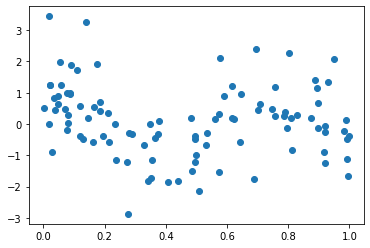
\includegraphics[width=.8\linewidth]{images/data.png}
            \caption{Data}
            \label{data}
        \end{subfigure}
        \hfill
        \begin{subfigure}{.5\textwidth}
            \centering
            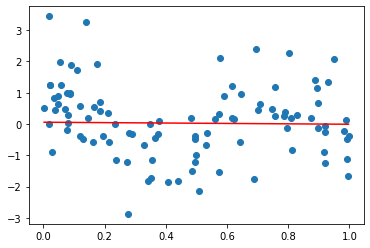
\includegraphics[width=.8\linewidth]{images/data-1.png}
            \caption{Linear model}
            \label{linear}
        \end{subfigure}
        \hfill
        \begin{subfigure}{.5\textwidth}
            \centering
            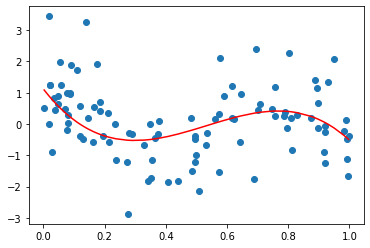
\includegraphics[width=.8\linewidth]{images/data-3.png}
            \caption{Third order model}
            \label{third}
        \end{subfigure}
        \begin{subfigure}{.5\textwidth}
            \centering
            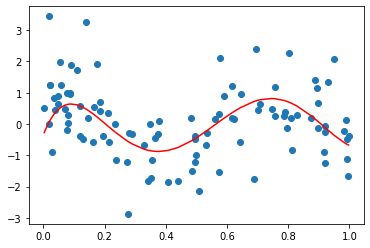
\includegraphics[width=.8\linewidth]{images/data-5.png}
            \caption{Fifth order model}
            \label{fifth}
        \end{subfigure}
        \caption{Training result of different models}
        \label{fig:model}
    \end{figure}
    Compare the linear model with the fifth order model, the linear model has lower error than the fifth order model.

    \item Generate a sample from a multivariate normal density $N(\mu, \Sigma)$, calculate $m$ and $S$, and compare them with $\mu$ and $\Sigma$. Check how your estimates change as the sample size changes. (Ch5 Ex2) % Ch5 Ex2
    
    \textbf{Answer:} \\
    I generated samples that follow multivariate normal using the \emph{numpy} package in Python. 
    The parameters I used to generate samples are 
    $$
    \mu=[5, 2], \Sigma=
    \left[\begin{array}{ll}
    6 & -3 \\
    -3 & 3.5
    \end{array}\right]
    $$
    After generation, the sample mean $m$ is computed by $\frac{1}{n}\sum^n_{i=1} x_i$ using the np.mean function, the sample covariance is computed by $\frac{1}{n-1}\sum_{i=1}^n (x_i-\bar x)(y_i-\bar y)$ using the np.cov function. 
    When $n=10$:\\
    $$
    m = [6.33, 1.24], S = 
    \left[\begin{array}{ll}
        2.94 & -0.23 \\
        -0.23 & 1.34
        \end{array}\right]
    $$
    When $n=100$:\\
    $$
    m = [5.53, 1.68], S = 
    \left[\begin{array}{ll}
        6.07 & -3.34 \\
        -3.34 & 4.14
        \end{array}\right]
    $$
    When $n=500$:\\
    $$
    m = [5.15, 1.93], S = 
    \left[\begin{array}{ll}
        6.04 & -2.80 \\
        -2.80 & 3.52
        \end{array}\right]
    $$
    When $n=1000$:\\
    $$
    m = [4.96, 2.04], S = 
    \left[\begin{array}{ll}
        5.97 & -2.81 \\
        -2.81 & 3.14
        \end{array}\right]
    $$
    When $n=5000$:\\
    $$
    m = [5.02, 2.00], S = 
    \left[\begin{array}{ll}
        6.09 & -2.96 \\
        -2.96 & 3.44
        \end{array}\right]
    $$
    We can see clearly that as n increases, the estimate values $m, S$ become generally closer to $\mu$ and $\Sigma$.

    \item  Generate samples from two multivariate normal densities $N\sim(\mu_i, \Sigma_i)$, i = 1, 2, and calculate the Bayes’ optimal discriminant for the four cases in table 5.1. (Ch5 Ex3)% Ch5 Ex3 (Correspond to p100 #122 in the textbook)
    \begin{center}
        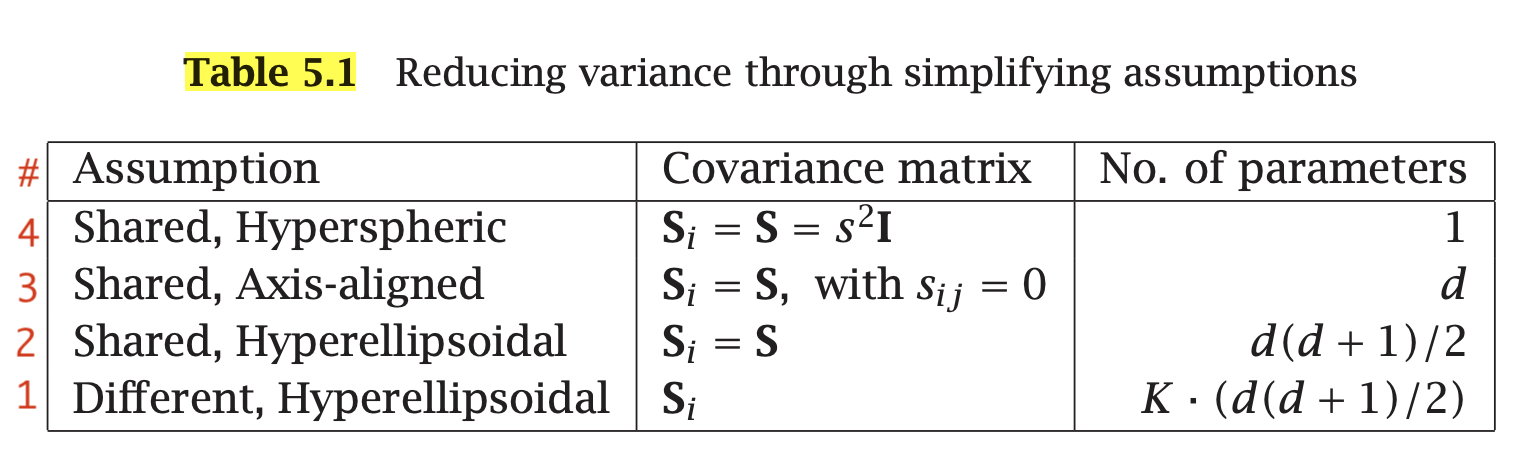
\includegraphics[width=0.8\linewidth]{table5.1.png}
    \end{center}
    \textbf{Answer:} 
    Since samples are taken from $N_i(\mu_i, \Sigma_i), i=1,2$,
    $$
    p\left(\boldsymbol{x} \mid C_i\right)=\frac{1}{(2 \pi)^{d / 2}\left|\boldsymbol{\Sigma}_i\right|^{1 / 2}} \exp \left[-\frac{1}{2}\left(\boldsymbol{x}-\boldsymbol{\mu}_i\right)^T \boldsymbol{\Sigma}_i^{-1}\left(\boldsymbol{x}-\boldsymbol{\mu}_i\right)\right]
    $$
    The Bayes' discriminant is 
    $$
    g_i(\boldsymbol{x})=\log p\left(\boldsymbol{x} \mid C_i\right)+\log P\left(C_i\right)
    $$
    $$
    g_i(\boldsymbol{x})=-\frac{d}{2} \log 2 \pi-\frac{1}{2} \log \left|\Sigma_i\right|-\frac{1}{2}\left(\boldsymbol{x}-\boldsymbol{\mu}_i\right)^T \boldsymbol{\Sigma}_i^{-1}\left(\boldsymbol{x}-\boldsymbol{\mu}_i\right)+\log P\left(C_i\right)
    $$
    While
    $$
    \begin{aligned}
    \hat{P}\left(C_i\right) &=\frac{\sum_t r_i^t}{N} \\
    \boldsymbol{m}_i &=\frac{\sum_t r_i^t \boldsymbol{x}^t}{\sum_t r_i^t} \\
    \mathbf{S}_i &=\frac{\sum_t r_i^t\left(\boldsymbol{x}^t-\boldsymbol{m}_i\right)\left(\boldsymbol{x}^t-\boldsymbol{m}_i\right)^T}{\sum_t r_i^t}
    \end{aligned}
    $$
    With Assumption \#1, after removing the constant term, the discriminant becomes follows (also Figure~\ref{fig:disc}(a)).
    $$
    g_i(\boldsymbol{x})=-\frac{1}{2} \log \left|S_i\right|-\frac{1}{2}\left(\boldsymbol{x}-\boldsymbol{m}_i\right)^T \boldsymbol{S}_i^{-1}\left(\boldsymbol{x}-\boldsymbol{m}_i\right)+\log P\left(C_i\right)
    $$
    This function defines a quadratic discriminant.

    With Assumption \#2, with a some covariance matrix, the discriminant becomes follows (also Figure~\ref{fig:disc}(b)).
    $$
    g_i(\boldsymbol{x})=-\frac{1}{2}\left(\boldsymbol{x}-\boldsymbol{m}_i\right)^T \mathbf{S}^{-1}\left(\boldsymbol{x}-\boldsymbol{m}_i\right)+\log \hat{P}\left(C_i\right)
    $$
    This function defines a linear discriminant.

    With Assumption \#3, all off-diagonal terms set to be 0, the discriminant becomes follows (also Figure~\ref{fig:disc}(c)).
    $$
    g_i(\boldsymbol{x})=-\frac{1}{2} \sum_{j=1}^d\left(\frac{x_j^t-m_{i j}}{s_j}\right)^2+\log \hat{P}\left(C_i\right)
    $$
    With Assumption \#4, all off-diagonal terms set to be 0, and the diagonal term (variances) are equal, the discriminant becomes follows (also Figure~\ref{fig:disc}(d)).
    $$
    g_i(\boldsymbol{x})=-\frac{\left\|\boldsymbol{x}-\boldsymbol{m}_i\right\|^2}{2 s^2}+\log \hat{P}\left(C_i\right)=-\frac{1}{2 s^2} \sum_{j=1}^d\left(x_j^t-m_{i j}\right)^2+\log \hat{P}\left(C_i\right)
    $$
    \begin{figure}[h!]
        \centering
        \begin{subfigure}[b]{0.45\textwidth}
            \centering
            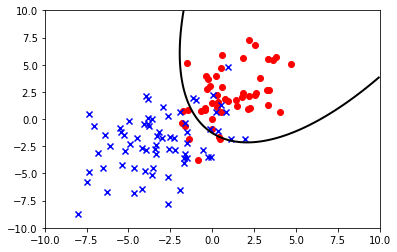
\includegraphics[width=\textwidth]{images/assump1.png}
            \caption{Assumption \#1 Unequal Covariance}
            \label{fig:assump1}
        \end{subfigure}
        \hfill
        \begin{subfigure}[b]{0.45\textwidth}
            \centering
            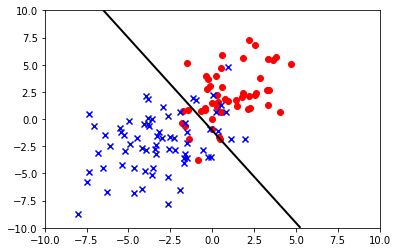
\includegraphics[width=\textwidth]{images/assump2.png}
            \caption{Assumption \#2 Equal Covariance}
            \label{fig:assump2}
        \end{subfigure}
\end{figure}
\begin{figure}[h!]
    \centering
    \begin{subfigure}[b]{0.45\textwidth}
        \centering
        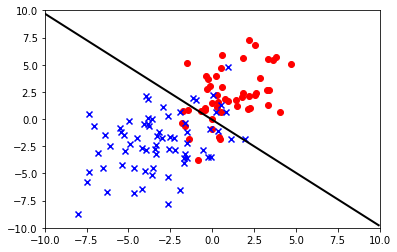
\includegraphics[width=\textwidth]{images/assump3.png}
        \caption{Assumption \#3 Independence}
        \label{fig:assump3}
    \end{subfigure}
    \hfill
    \begin{subfigure}[b]{0.45\textwidth}
        \centering
        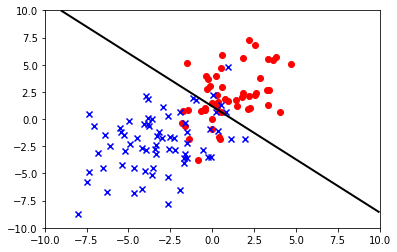
\includegraphics[width=\textwidth]{images/assump4.png}
        \caption{Assumption \#4 Equal variance}
        \label{fig:assump4}
    \end{subfigure}
    \caption{Bayes' discriminants of different assumptions}
    \label{fig:disc}
\end{figure}
    

    \item  In figure 6.11, we see a synthetic two-dimensional data where LDA does a better job than PCA. Draw a similar dataset where PCA and LDA find the same good direction. Draw another where neither PCA nor LDA find a good direction.\\ % Ch6 Ex5
    \begin{center}
        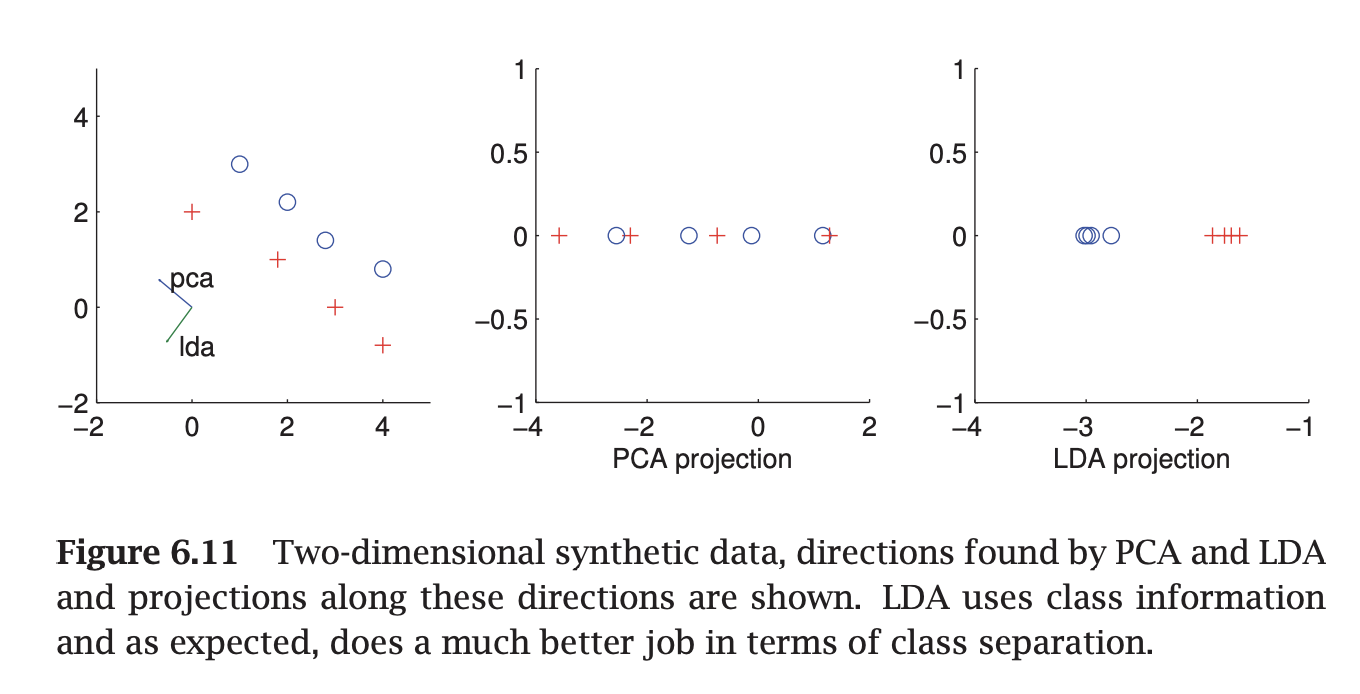
\includegraphics[width=0.95\linewidth]{figure 6-11.png}
    \end{center}
    
    \textbf{Answer:} \\
    This is the case where LDA and PCA find the same good direction.
    \begin{center}
        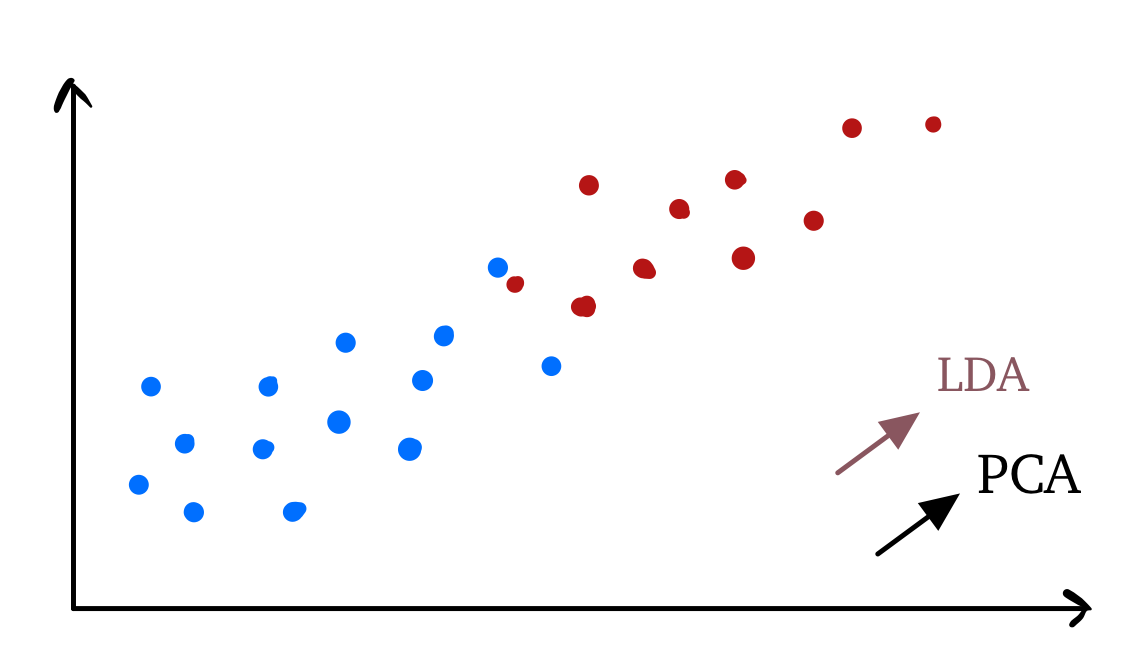
\includegraphics[width=0.6\linewidth]{q7-1.png}
    \end{center}
    
    Since PCA and LDA are both linear transformers. When the boundary of data is not linear, neither PCA nor LDA can find a good direction.
    \begin{center}
        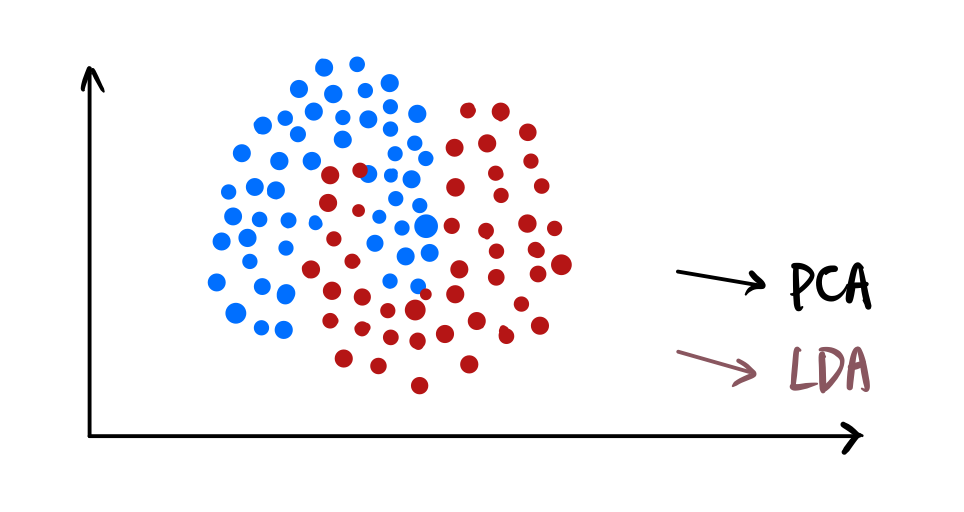
\includegraphics[width=0.6\linewidth]{q7-2.png}
    \end{center}


\end{enumerate}
\end{document}